\section{Regler}
\subsection{Schaltenderegler}
\subsubsection{Zweipunkte-Regler}\script{64}
Ein Zweipunktregler ist ein unstetig arbeitender Regler mit zwei Ausgangszuständen ($a,b$). Je nachdem,
ob der Ist-Wert über oder unter dem Soll-Wert liegt, wird der erste oder der zweite Ausgangszustand
eingenommen.~\\

\noindent Um eine \textbf{Kennlinie} (X-Y-Plot) zu zeichnen, können den Signalen \textcolor{green}{$x(t)$}  \textcolor{red}{$y(t)$} verfolgt und geplotet werden.
\begin{center}
	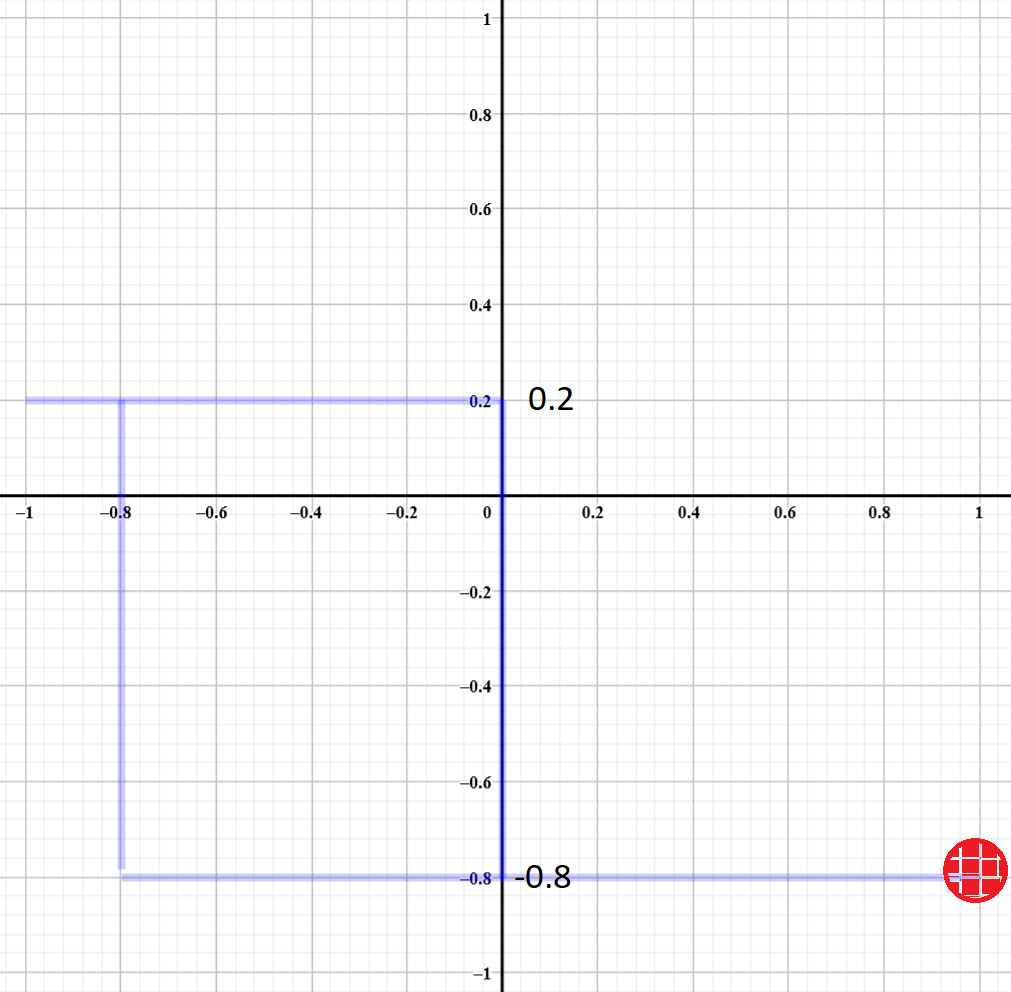
\includegraphics[width=0.3\columnwidth]{Images/kennlinie}
	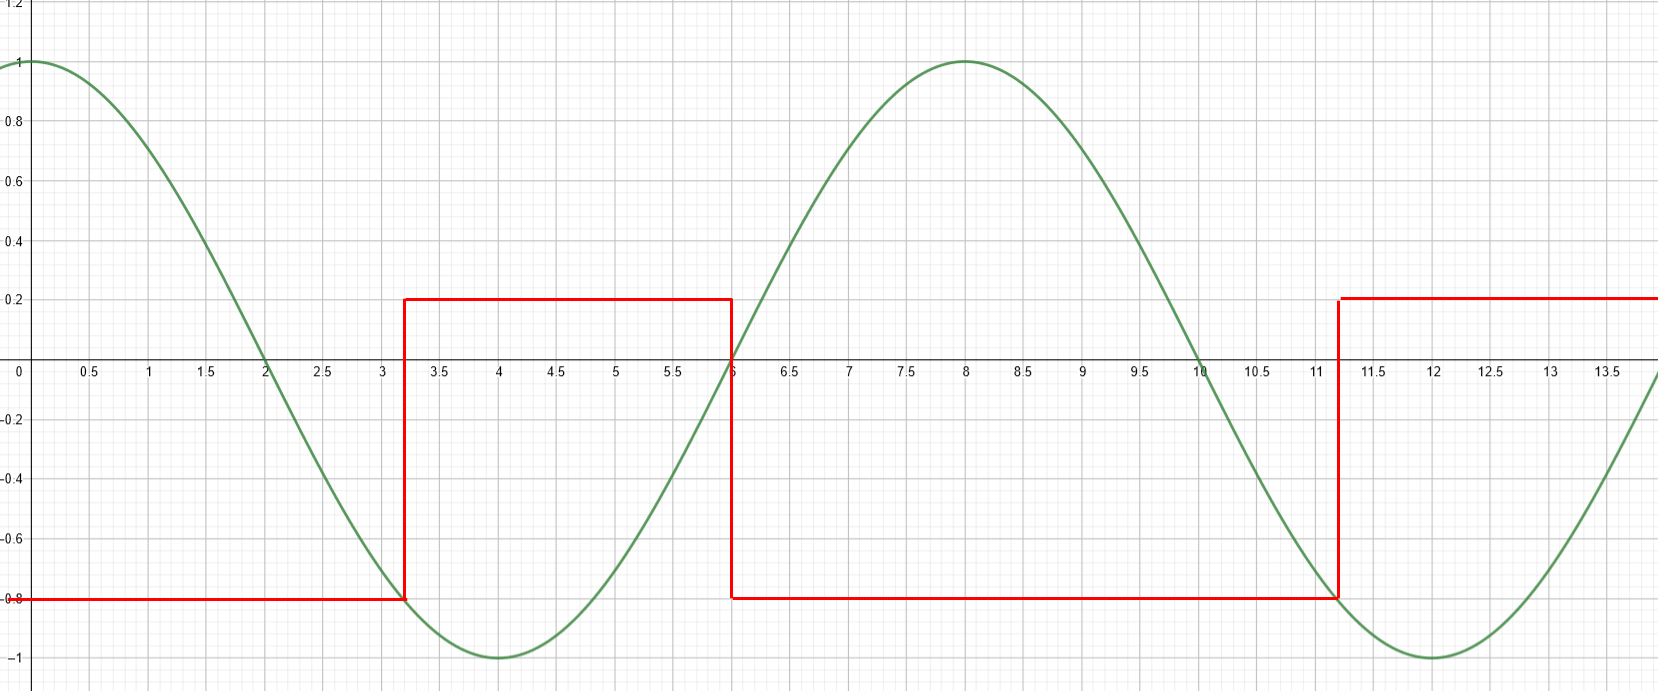
\includegraphics[width=0.6\columnwidth]{Images/zweipunkte-regler}
\end{center}

\noindent Anfang für Beispiel von oben bei $x(t = 0) = 1$ und $y(t = 0) = -0.8$ (roter Punkt), dann $t\rightarrow\infty$. Dabei entsteht eine Hysterkennlinie.

\subsubsection{Dreipunkt-Regler}\script{70}
Im Gegensatz zum Zweipunktregler gibt es im Dreipunktregler eine Ruhelage. Dies ist eine Kompination aus zwei Zweipunktregler.\\
\begin{center}
	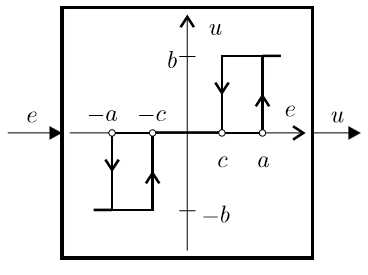
\includegraphics[width=0.3\columnwidth]{Images/dreipunktregler}
\end{center}

\textbf{Beispiel Konvertierung}
\begin{center}
	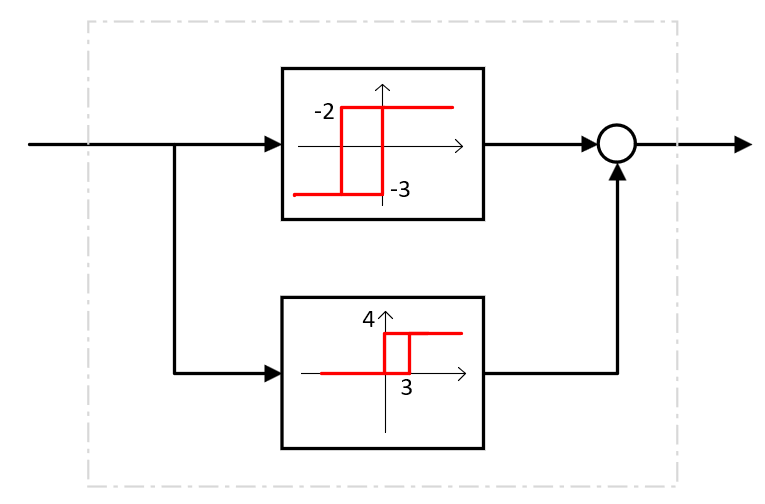
\includegraphics[width=0.5\columnwidth]{Images/3pr_I}
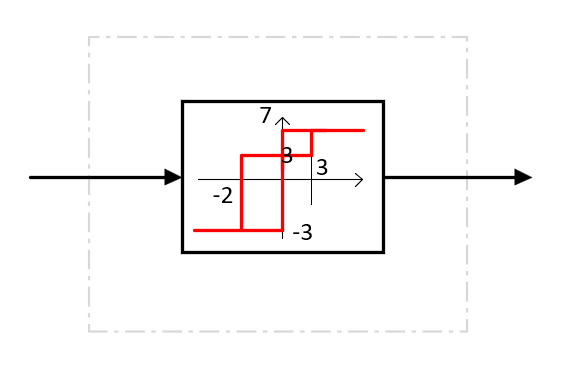
\includegraphics[width=0.4\columnwidth]{Images/3pr_II}
\end{center}


\subsection{Stetigähnlicher Regler}\script{71}
Sind spezielle Regler, welche modifizierte Schaltenderegler sind. Gegenüber schaltenden Reglner sind stetigähnliche Regler also aufwendiger zu bauen, aber am Regerausgang ändert sich nicht viel.